\section{Resultados}
Una vez implementados el algoritmo genético y sus dos variantes, lo ejecutamos usando los datos del fichero \textit{tai256c} proporcionado, obteniendo los siguientes resultados:

\begin{table}[H]
\centering
\begin{tabular}{|l|l|l|l|l|}
\hline
Variante & Población & Generaciones & Coste & Tiempo (s) \\ \hline
Base & 100 & 1000 & 45022826 & 3.46 \\ \hline
Baldwiniana & 100 & 150 & 44965852 & 97.36 \\ \hline
Lamarckiana & 100 & 150 & 44920302 & 102.66 \\ \hline
\end{tabular}
\end{table}

Como se puede apreciar, al introducir heurísticas el tiempo de ejecución del algoritmo aumenta considerablemente, pero también obtenemos mejores resultados en un número mucho menor de generaciones que con el algoritmo base, cosa que se puede apreciar mejor en la siguiente gráfica, la cuál muestra la evolución del coste del mejor individuo a lo largo de las generaciones.

\begin{figure}[H]
\centering
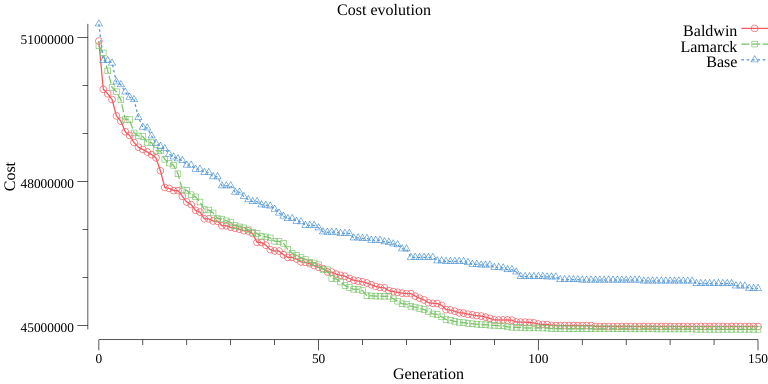
\includegraphics[width=\textwidth]{images/costEvolution.png}
\end{figure}

El mejor resultado lo obtenemos con la variante lamarckiana, aunque su funcionamiento tampoco es mucho mejor que el de la variante baldwiniana, cosa que se puede comprobar en la gráfica.